\documentclass[twocolumn]{article}
\usepackage[top=1.1in, left=0.85in, right=0.85in]{geometry}

\usepackage{code}
\usepackage{cite}
% \usepackage{eclbkbox}
\usepackage{amsmath}
\usepackage{amssymb}
% \usepackage{code}
% \usepackage{amscd}
% \usepackage{xy}
\usepackage{graphicx}
% \usepackage{fancyhdr}
% \usepackage{color}
% \usepackage[dark,all,bottom,landscape,timestamp]{draftcopy}
% \usepackage{everypage}

% \pagestyle{empty}

\usepackage{ulem}
% go back to italics for emphasis, though
\normalem

% \usepackage{inlinebib}

\newcommand\comment[1]{}
\newcommand\sfrac[2]{{}\,^{#1}\!/{}\!_{#2}}

\begin{document} 

\title{New results in $\sfrac{k}{n}$ Power-Hours}
\author{Dr.~Tom~Murphy~VII~Ph.D.\thanks{
Copyright \copyright\ 2014 the Regents of the Wikiplia
Foundation. Appears in SIGBOVIK 2014 with the chagrin of the
Association for Computational Heresy; {\em IEEEEEE!} press,
Verlag-Verlag volume no.~0x40-2A.
\yen 0.00}
}

\renewcommand\th{\ensuremath{{}^{\textrm{th}}}}
\newcommand\st{\ensuremath{{}^{\textrm{st}}}}
\newcommand\rd{\ensuremath{{}^{\textrm{rd}}}}
\newcommand\nd{\ensuremath{{}^{\textrm{nd}}}}
\newcommand\at{\ensuremath{\scriptstyle @}}

\renewcommand\>{$>$}
\newcommand\<{$<$}
\newcommand\kn{\ensuremath{\sfrac{k}{n}\,}}

\newcommand\any{\ensuremath{\textrm{?}}}
\newcommand\nocup{\text{\sout{\ensuremath{\cup}}}}
\newcommand\fullcup{\ensuremath{\uplus}}
\newcommand\emptycup{\ensuremath{\cup}}
\newcommand\overcup{\ensuremath{\cap}}

\newcommand\nodrink{\ensuremath{\Rightarrow}}
\newcommand\drink{\ensuremath{\stackrel{{}^{\textrm{+}}}{\Rightarrow}}}
\newcommand\qdrink{\ensuremath{\stackrel{{}^{\textrm{?}}}{\Rightarrow}}}

\date{1 April 2014}

\maketitle

\begin{abstract}
Something about the k-n hours

\end{abstract}

\vspace{1em}
{\noindent \small {\bf Keywords}:
  generalized binge drinking, maths,
  finite-state automata,
  abstract interpretation
}

\section*{Introduction}
A 2012 paper by Blum, Martens, Murphy, and Lovas\cite{algorithms}
introduced the \kn Power-Hour, a fractional variant on the well-known
drinking game. In a traditional Power-Hour, participants drink one
shot of beer per minute for 60 minutes. Since 5--6 beers in an hour
sometimes have adverse effects, some players opt for an attenuated
version of the game wherein fewer than 60 shots are consumed. However,
since the game is frantic and played simultaneous with others, it is
critical to have a mechanical procedure for performing the attenuated
Hour. The framework by Blum {\em et al.}, hereafter BMML, gives a
handful of simple operations that can be used to define a state
machine among $p$ players:
\begin{itemize}
  \item At the beginning of each minute, each player has at most one
    shot glass in front of him or her
  \item The shot glass must be in one of three states: Filled \fullcup,
    empty \emptycup, or overturned \overcup
  \item Atomically, each player performs an action based only on the
    state of his or her cup. If not in possession of a cup (written
    \nocup), the only action is to do nothing. With a cup:
  \begin{itemize}
    \item The player may drink \drink, or not drink \nodrink
    \item The player may pass the cup in any state to any player (a
      fixed player per action)
    \item However: If the cup is filled and the player did not drink,
      it must be passed in the filled state
    \item A player may not receive more than one cup in the same round
  \end{itemize}
\end{itemize}

Every assignment of rules and starting condition to $p$ players yields
a deterministic outcome, though some of these are illegal (because
they result in two or more cups being passed to the same player in
some round). For legal games, the outcome is that the $p$ players have
consumed $k_i$ shots of beer where $1 \leq i \leq p$ and $0 \leq k_i
\leq 60$. For the traditional power hour, the player starts with an
empty cup, at each step drinks,\!\footnote{In practice, this is done
  by filling the cup and then drinking it.} leaves the cup empty, and
passes to herself.

While the authors made a mostly clear definition of BMML and presented
some initial results, these results contained multiple serious errors
and the paper abruptly switches notation and assumptions several
times, and rambles incoherently. By their own admission, the authors
were drinking while they wrote it, taking only one hour to do so.
Don't drink and derive, kids!

This paper revisits the problem of BMML from a modern, sober
perspective, clarifies some of the original results, and presents
several new ones and a few conjectures.

\section{One-player \kn Power-Hours}

The goal of the \kn Power-Hour is to attenuate the number of drinks
consumed by the $p$ players, and its expressive power comes from the
ability to encode some state in the orientation of the cups, and
propagate that state via passing them from player to player. Even
without passing cups, the ability for a single player to attenuate his
drinking is nontrivial. Playing drinking games alone is sad indeed,
but the solo \kn Power-Hour still has practical applications. When
playing a Power Hour with others, if each player's desired $k$ is
attainable through solo methods then there is no need for passing
cups, which simplifies the ergonomics considerably. A common case is
where some of the players would like to do half--Power-Hours, which is
easily achieved in BMML by transitioning \emptycup\ to \fullcup\ without
drinking and \fullcup\ to \emptycup\ by drinking, and passing to
oneself.\!\footnote{There are many variations, but this was the
  strategy used many times in practice before being generalized to
  BMML.}

A full list of attainable \kn Power-Hours where $p=1$ appears in
Figure~\ref{fig:solo}. Possible values of $k$ are $\{ 0, 1, 2, 20, 29,
30, 31, 40, 58, 59, 60 \}$. The BMML paper claimed that the possible
values were $\{0, 1, 2, 20, 30, 40, 58, 59, 60 \}$, describing 31 for
example as ``super impossible.'' Achieving 31 is somewhat interesting.
One way to do it is to start with \emptycup, and use the rule that
\emptycup\ means drink and then fill the cup. We then use the rule
that \fullcup\ means drink and flip the cup, and \overcup\ means don't
drink and fill the cup. Essentially we use \emptycup\ to mean ``this
is the very first state'' and then take shots on alternating minutes
by using \overcup\ and \fullcup\ to encode the parity. Exploiting
non-steady-states like this (Figure~\ref{fig:solo31}) is how we
achieve $k$ that does not divide $n$.

\begin{figure}[ht]
\begin{center}
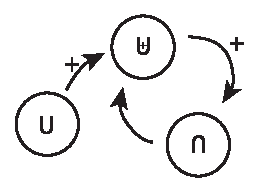
\includegraphics[width=0.90 \linewidth]{solo31.pdf}
\end{center}\vspace{-0.1in}
\caption{State machine that achieves $k=31$ in a solo BMML Power Hour.
  $+$ on an edge means the player drinks. The disembodied incoming
  edge is the start state. The player always passes to herself.}
\label{fig:solo31}
\end{figure}

It is tractable to work out the possibilities for the solo case by
hand, though apparently not while drinking~\cite{algorithms}. These
results were generated by a computer program, which is probably
necessary for $p>1$. The next section describes how we explore this
space computationally. XXX no it doesn't

\begin{figure}[ht]
\begin{center}
\begin{tabular}{c|ll}
$k$ & start & rules \\
\hline
0  &   \nocup    &  \emptycup \nodrink \any     , \overcup \nodrink \any      , \fullcup \nodrink \any \\
1  &   \emptycup &  \emptycup \drink \overcup   , \overcup \nodrink \overcup  , \fullcup \nodrink \any \\
2  &   \emptycup &  \emptycup \drink \fullcup   , \overcup \nodrink \overcup  , \fullcup \drink \overcup \\
20 &   \emptycup &  \emptycup \nodrink \overcup , \overcup \nodrink \fullcup  , \fullcup \drink \emptycup \\
29 &   \emptycup &  \emptycup \nodrink \overcup , \overcup \nodrink \fullcup  , \fullcup \drink \overcup \\
30 &   \emptycup &  \emptycup \drink \overcup   , \overcup \nodrink \emptycup , \fullcup \nodrink \any \\
31 &   \emptycup &  \emptycup \drink \fullcup   , \overcup \nodrink \fullcup  , \fullcup \drink \overcup \\
40 &   \emptycup &  \emptycup \drink \overcup   , \overcup \nodrink \fullcup  , \fullcup \drink \emptycup \\
58 &   \emptycup &  \emptycup \nodrink \overcup , \overcup \nodrink \fullcup  , \fullcup \drink \fullcup \\
59 &   \emptycup &  \emptycup \nodrink \overcup , \overcup \drink \overcup    , \fullcup \nodrink \any \\
60 &   \emptycup &  \emptycup \drink \emptycup  , \overcup \nodrink \any      , \fullcup \nodrink \any \\
\end{tabular}
\end{center}
\label{fig:solo}
\caption{All the possible $k$ for a solo Power-Hour in BMML. A
  superscript $+$ means that the player drinks. The symbol \any\ means
  that any cup state can be used in that position. Note that 29 and 58
  require wasting a shot of beer; all the others but 31 permit a
  variant where a shot is wasted as well.}
\end{figure}

\section{Two-player \kn Power-Hours}

For more players, the number of possible configurations explodes.
Let's make the following definitions to bound the size:
\begin{itemize}
\item $s = 4$, the number of starting states (\fullcup, \emptycup,
  \overcup, \nocup)
\item $a = 2 * p * 3$, the number of actions given a cup. The player
  can drink or not drink, pass to any player, and in 3 configurations
  (\fullcup, \emptycup, \overcup)
\end{itemize}
Then the number of configurations is bounded by $(s * a^3)^p$. For
$p=1$ this was just 864. For $p=2$ it is 47,775,744; for $p=3$ it's
12,694,994,583,552, already beyond the limits of straight enumeration.

\comment{
fun ct (p : IntInf.int) =
  let val s = 4
      fun pow n 0 = 1
        | pow n m = n * pow n (m - 1)
      val a = 2 * p * 3
   in
      pow (s * pow a 3) p
  end
}

However, this is just an upper bound. For one thing, the base of the
exponent is actually bounded by
$$
  s * a^2 * a_{\textrm{filled}}
$$
where
$a_{\textrm{filled}} = (p * 3) + p$ (the actions that can be taken on
\fullcup, where if the player does not drink, then he must pass the
cup \fullcup).

\comment{
fun ctb (p : IntInf.int) =
  let val s = 4
      fun pow n 0 = 1
        | pow n m = n * pow n (m - 1)
      val af = p * 3 + p
      val a = 2 * p * 3
   in
      pow (s * pow a 2 * af) p
  end
}

The values for $p \in \{1,2,3\}$ are still 576; 21,233,664;
3,761,479,876,608. There are a few other simplifications possible.
Many of these games are illegal because they result in multiple cups
being passed to the same player in some turn. These are difficult to
exclude analytically, but there are some sufficient conditions; for
example, if two players pass to the same player no matter their input
state, then their cups always collide. There are also many games
that are isomorphic. For one thing, \emptycup\ and \overcup\ are not
distinguished in the rules at all, so any two configurations where
these are simply swapped has the exact same outcome. Likewise for
permuting the players.

21 million configurations is no big deal for a modern computer. A
simple SML program computes all of the configurations and runs them;
ones that are found to be illegal are rejected. (It implements the
first simplification having to do with \fullcup\ when generating the
configurations, since it can be done statically.) All of the possible
outcomes are shown as black squares in Figure~\ref{fig:powerhour2player}.

\begin{figure}[ht]
\begin{center}
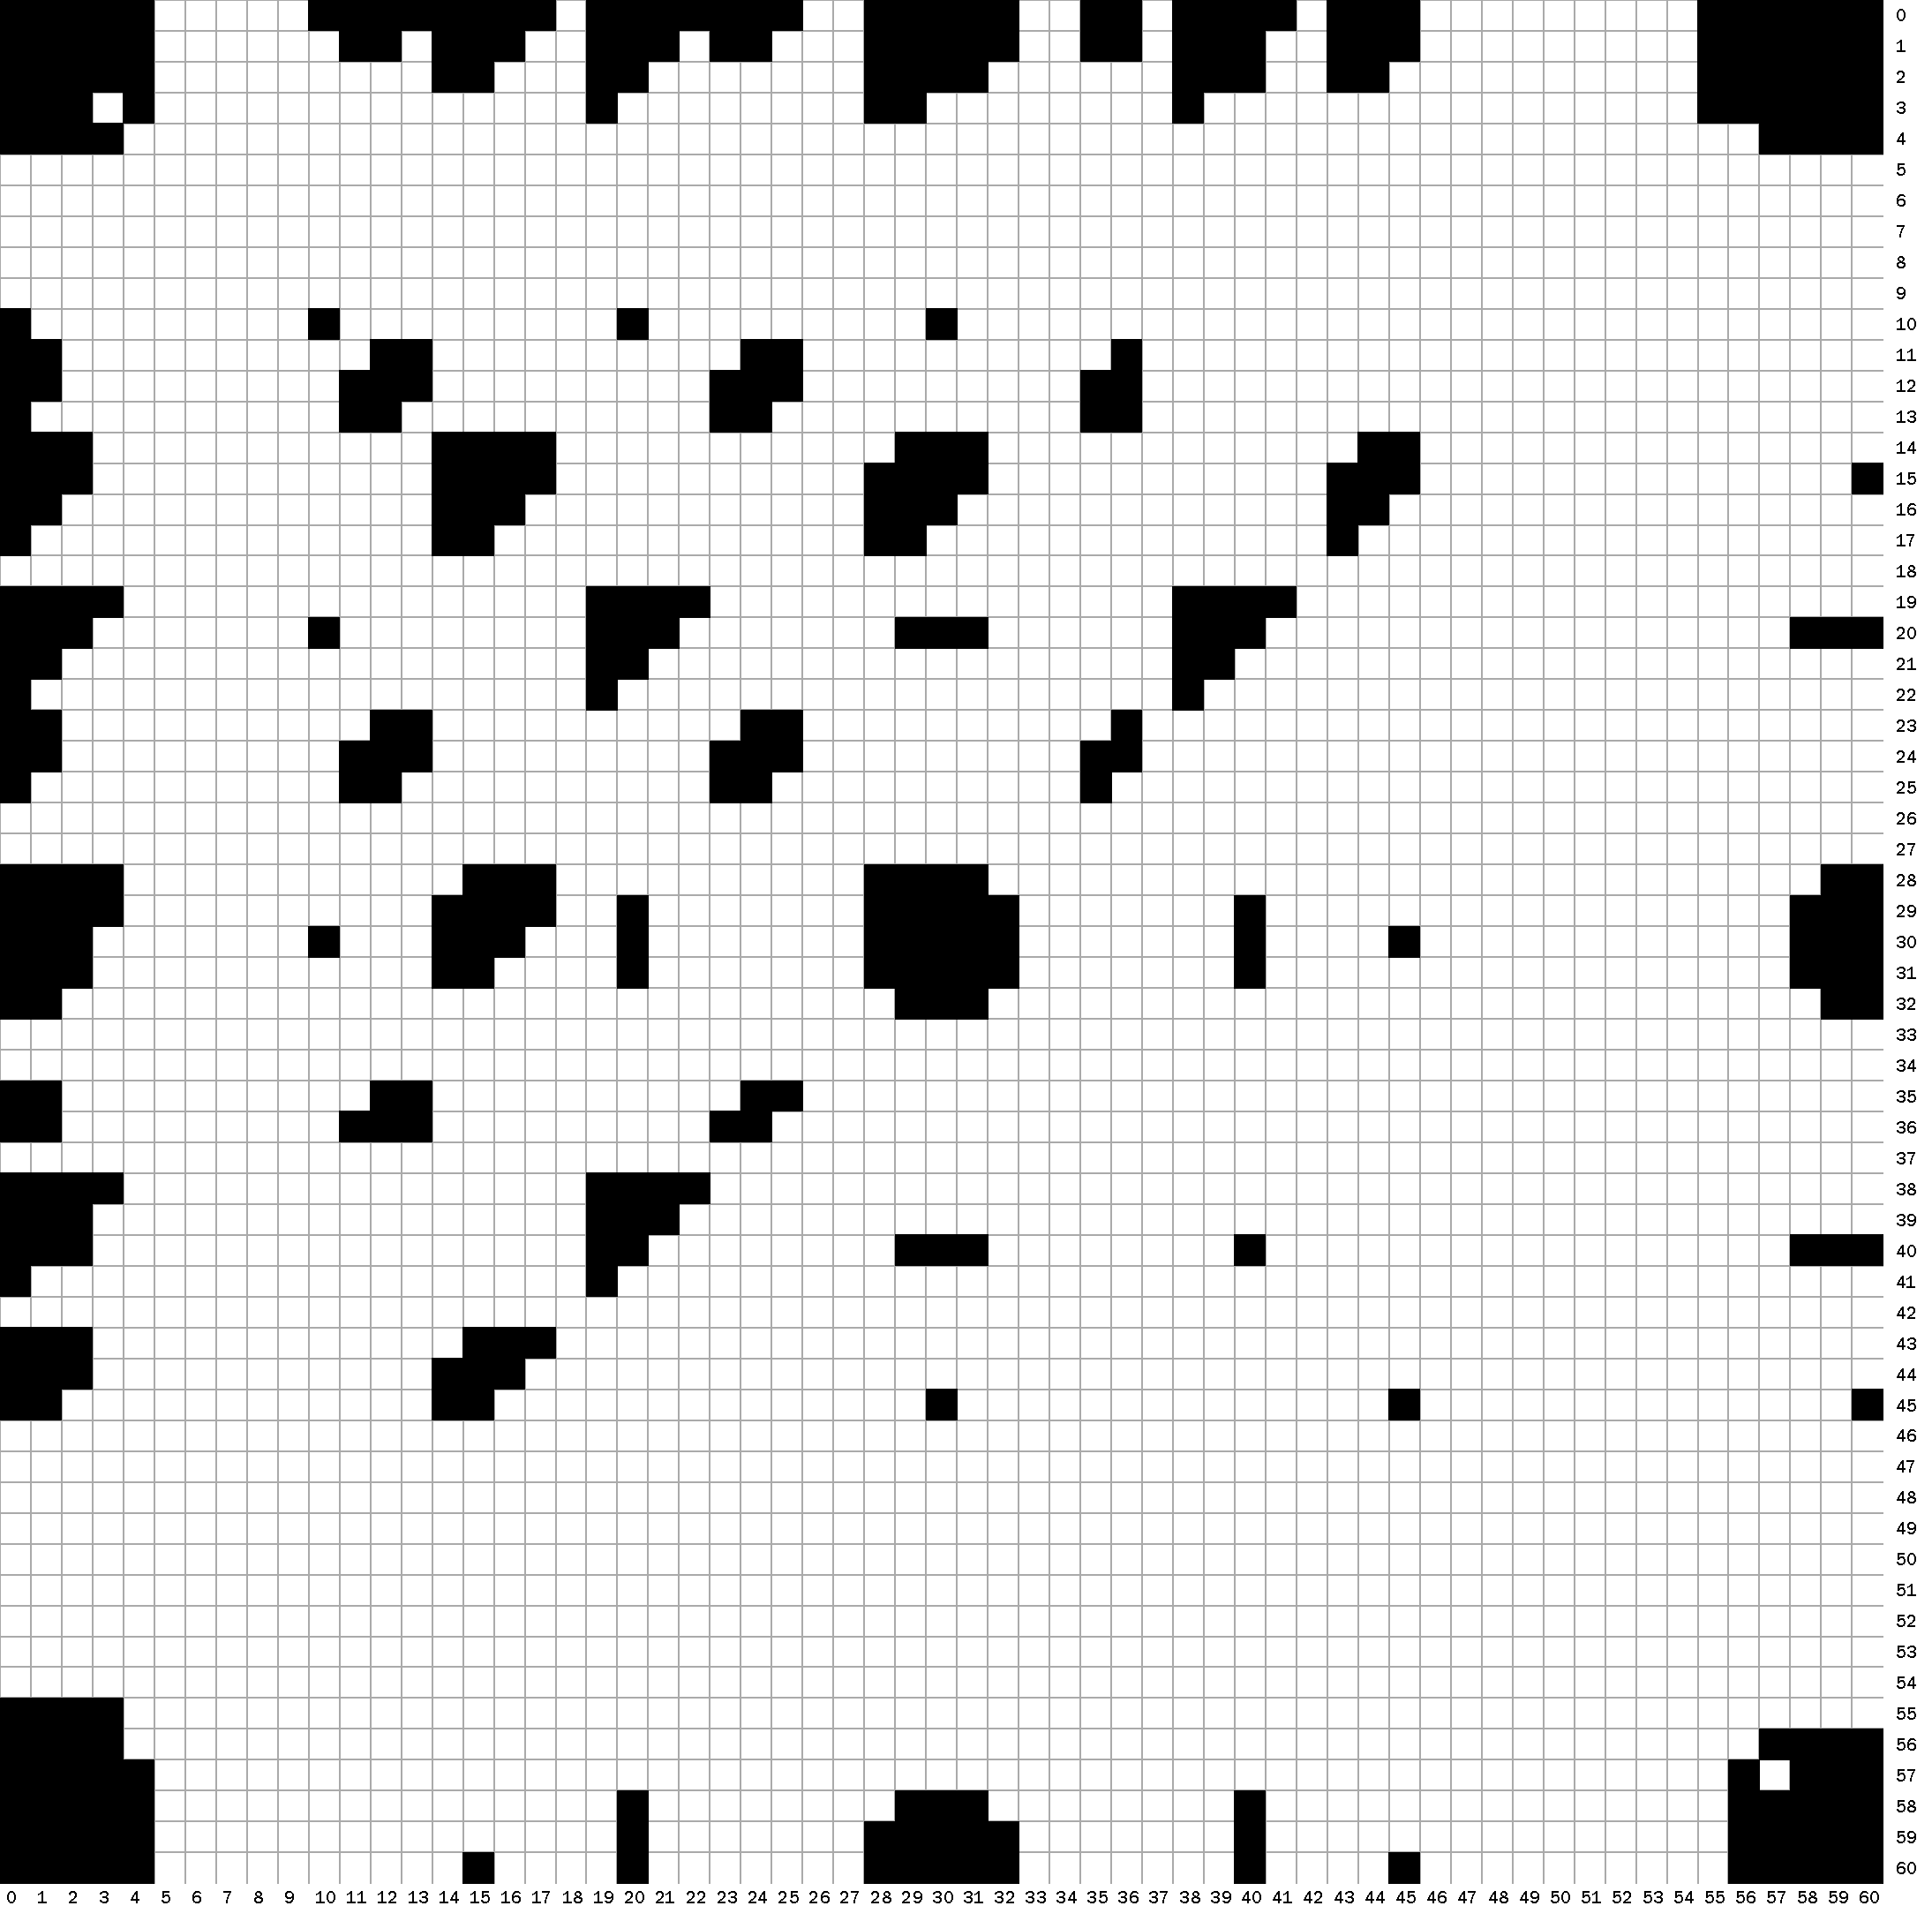
\includegraphics[width=0.90 \linewidth]{powerhour2player.pdf}
\end{center}\vspace{-0.1in}
\caption{All of the possible outcomes ($k$) for the two players in a
  BMML Power-Hour. The matrix is symmetric, of course, since the players
  are interchangeable.}
\label{fig:powerhour2player}
\end{figure}

Each cell represents a pair of $\langle k_1, k_2 \rangle$ for the
number of shots imbibed by players 1 and 2. 454 of the $61^2 = 3721$
combinations are achievable. Note that column 0 represents the case
where player 1 drinks nothing. It dominates the matrix in the sense
that if $\langle k_1, k_2 \rangle$ is achievable, then $\langle 0, k_2
\rangle$ is as well. Most of the time it is easy to see how this is
done: Take the configuration that produces $\langle k_1, k_2 \rangle$
and do the same, but player 1 simply performs her actions without
drinking. This works except for the case where player 1 receives a
\fullcup\ and passes it in a state other than \fullcup. The player
can't simply not drink, as this is illegal (the beer must be emptied,
and BMML does not permit such messy reductions). It is curious that
this does not affect the result; I discuss this further in
Section~\ref{sec:conjectures}. Another interesting column is the last
one, which represents outcomes of the form $\langle 60, k_2 \rangle$,
where the first player achieves a full Power-Hour. This of course
includes all of the $k_2$ achievable solo (the players can just do
their thing without interacting). But some new $k$ are now achievable:
$\{ 3, 4, 15, 28, 32, 45, 56, 57 \}$. Interacting with a player doing
a full Power-Hour still affords us a few additional bits of
information that can be used to attenuate the other player's
consumption. The solution for $45$ is instructive, and appears in
Figure~\ref{fig:dual45}.

This is a useful result, but it may be the case that someone wants to
drink exactly 27 shots of beer, which is not possible with just two
players in BMML. There are two avenues to explore: Adding more 
players, and generalizing BMML. We begin with the three-player case.

\begin{figure}[ht]
\begin{center}
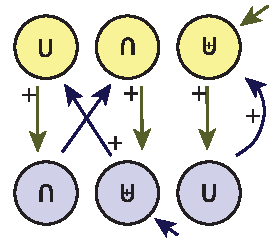
\includegraphics[width=0.90 \linewidth]{dual45.pdf}
\end{center}\vspace{-0.1in}
\caption{State machine that achieves $\langle k_1=45, k_2=60 \rangle$
  in a two-player BMML Power Hour. The bottom row of states are for
  player 1, who drinks 45, and the top for player 2, who drinks 60.
  Clearly, player 2 must drink at every step. The players always pass
  to each other, with the two cups exchanging hands each turn. The
  cycles for the two cups are disconnected; one alternates between
  \fullcup\ in player 2's hand and \emptycup\ in player 1's (cycle
  of length 2), drinking on each turn. This cycle yields 30 drinks
  for each player. The other cycle is of length 4; player 2 drinks
  on every step (as we know), and player 1 every 4\th\ step, yielding
  15 more drinks for a total of 45.
% [60,45] wasting 2: 12 game(s) like 
% [(start F, U=>D*@1 D=>F*@1 F=>U*@1),
%  (start F, U=>F*@0 D=>D@0 F=>U*@0)]
}
\label{fig:dual45}
\end{figure}

\section{Three-player \kn Power-Hours}

With 3.7 trillion possible configurations, enumeration is not
feasible. But as we observed before, many of these combinations are
illegal (they result in a player recieving two cups), and many are
isomorphic to one another. By being clever about how we explore the
configurations, testing ``all'' the three-player configurations
becomes feasible.

Here is a one-player BMML configuration that illustrates a particular
kind of redundancy:
\vspace{1em}
\begin{tabular}{cc}
start \emptycup & \emptycup \drink \emptycup 
 \quad \fullcup \drink \overcup
 \quad \overcup \nodrink \fullcup
\end{tabular}

The cup starts empty, and at each step the player fills it and drinks
(traditional Power-Hour). The player also has rules for the case that
she observes a full or overturned cup. {\em It does not matter what
  these are} because they can never be used. This example is trivial,
but there are many ways that the execution of a configuration can be
indifferent to some of its content. Another is a two player
configuration like
\vspace{1em}
\begin{tabular}{rcccc}
player 1 & start \emptycup & \emptycup \drink \overcup \at 1
 & \fullcup \drink \overcup \at 2
 & \overcup \nodrink \fullcup \at 1 \\
player 2 & start \emptycup & \emptycup \nodrink \emptycup \at 1
 & \fullcup \drink \overcup \at 1
 & \overcup \drink \fullcup \at 2 \\
\end{tabular}
where the $\at n$ notation means to pass the cup in that state to
player $n$. In this case, the first thing the players do is to
pass both of their cups to player 1, which is illegal and ends the
game. Again, none of the other rules are ever used.

In order to explore what is possible in three-player games, we exploit
this redundancy with a technique like abstract
interpretation~\cite{abstract}. The start state is always used, so we
begin by enumerating all assignments of start states to players. There
are only $4^p$. Every other rule starts out undetermined, maybe written
like this:

\begin{tabular}{cc}
start \emptycup & \emptycup \qdrink \any
 \quad \fullcup \qdrink \any
 \quad \overcup \qdrink \any
\end{tabular}

Now we execute programs as before, and hope that we never encounter a
situation where we depend on a rule. If we finish without ever using
one of the \any\ rules, we evaluated a potentially large group of
configurations all at once. During the execution of a configuration,
if we need to use a rule that is currently marked \any, we explore all
of the possibilities. This is accomplished by a loop that looks like
the following (in Pseudo SML):

\begin{code}
val queue = (* all abstract configurations *)
val results = (* map from (k_1, k_2) 
                 to example *)
\codeskip
fun loop nil = (* done *)
  | loop (h :: t) =
      let
        val res = evaluate h
      in
        insert (results, res);
        loop t
      end handle Expand l => loop (l @ t)
\codeskip
fun evaluate config =
   (* ... *) 
   case rulefor cup of 
      QuestionMark =>
         raise Expand expandedconfigs
    | (* ... *)
\codeskip
val () = loop queue
\end{code}

The key trick here for keeping the code under control is to
iteratively evaluate the configurations as usual, but if we find a
\any, then we abort the current simulation with an exception that
carries along the set of configurations that expand the current one in
just that position. This wastes some work (and we often need to
restart multiple times per abstract configuration), but not much: If a
rule is used at all, it is usually used in one of the first few
rounds.

With this technique, we can simulate all possible two-player games
with just 15,744,259 game-minutes simulated (with naive enumeration it
would be 1.2 billion) in less than 2 seconds on a crappy old computer.

% Total steps 15744259. Took 1982 ms
% Total steps 15744259. Took 2080 ms

% #100000 queue 31 min 16 6059166 states/sec 100000 config/sec
% #200000 queue 20 min 16 8762059 states/sec 200000 config/sec
% #300000 queue 35 min 16 12125162 states/sec 300000 config/sec
% #400000 queue 25 min 16 7613270 states/sec 200000 config/sec
% Total steps 15744259. Took 2101 ms

% There are 16 games before splitting.
% #100000 queue 31 min 16 6059166 states/sec 100000 config/sec
% #200000 queue 20 min 16 8762059 states/sec 200000 config/sec
% #300000 queue 35 min 16 6062581 states/sec 150000 config/sec
% #400000 queue 25 min 16 7613270 states/sec 200000 config/sec
% Wrote 454 possibilities to possible-2.txt
% Total steps 15744259. Took 2162 ms

% Wrote 454 possibilities to possible-2.txt
% Total steps 895743. Took 292 ms

% Wrote 2787 possibilities to possible-5cup-60min-2player.txt
% Total steps 6890640495. Took 8161324 ms

% on metroid
% Wrote 37560 possibilities to possible-3.txt
% Total steps 1393736865. Took 1,545,217 ms

\begin{figure}
\begin{center}

\includegraphics[width=0.90 \linewidth]{3and2.pdf}
\end{center}\vspace{-0.1in}
\caption{Outcomes possible for the first two players in all different
  3-player power hours (black), overlayed by all possible outcomes
  outcomes for 2-player power hours (red). Mainly included because
  it looks pretty sweet.
}
\label{fig:3and2}
\end{figure}

\begin{figure}
\begin{center}
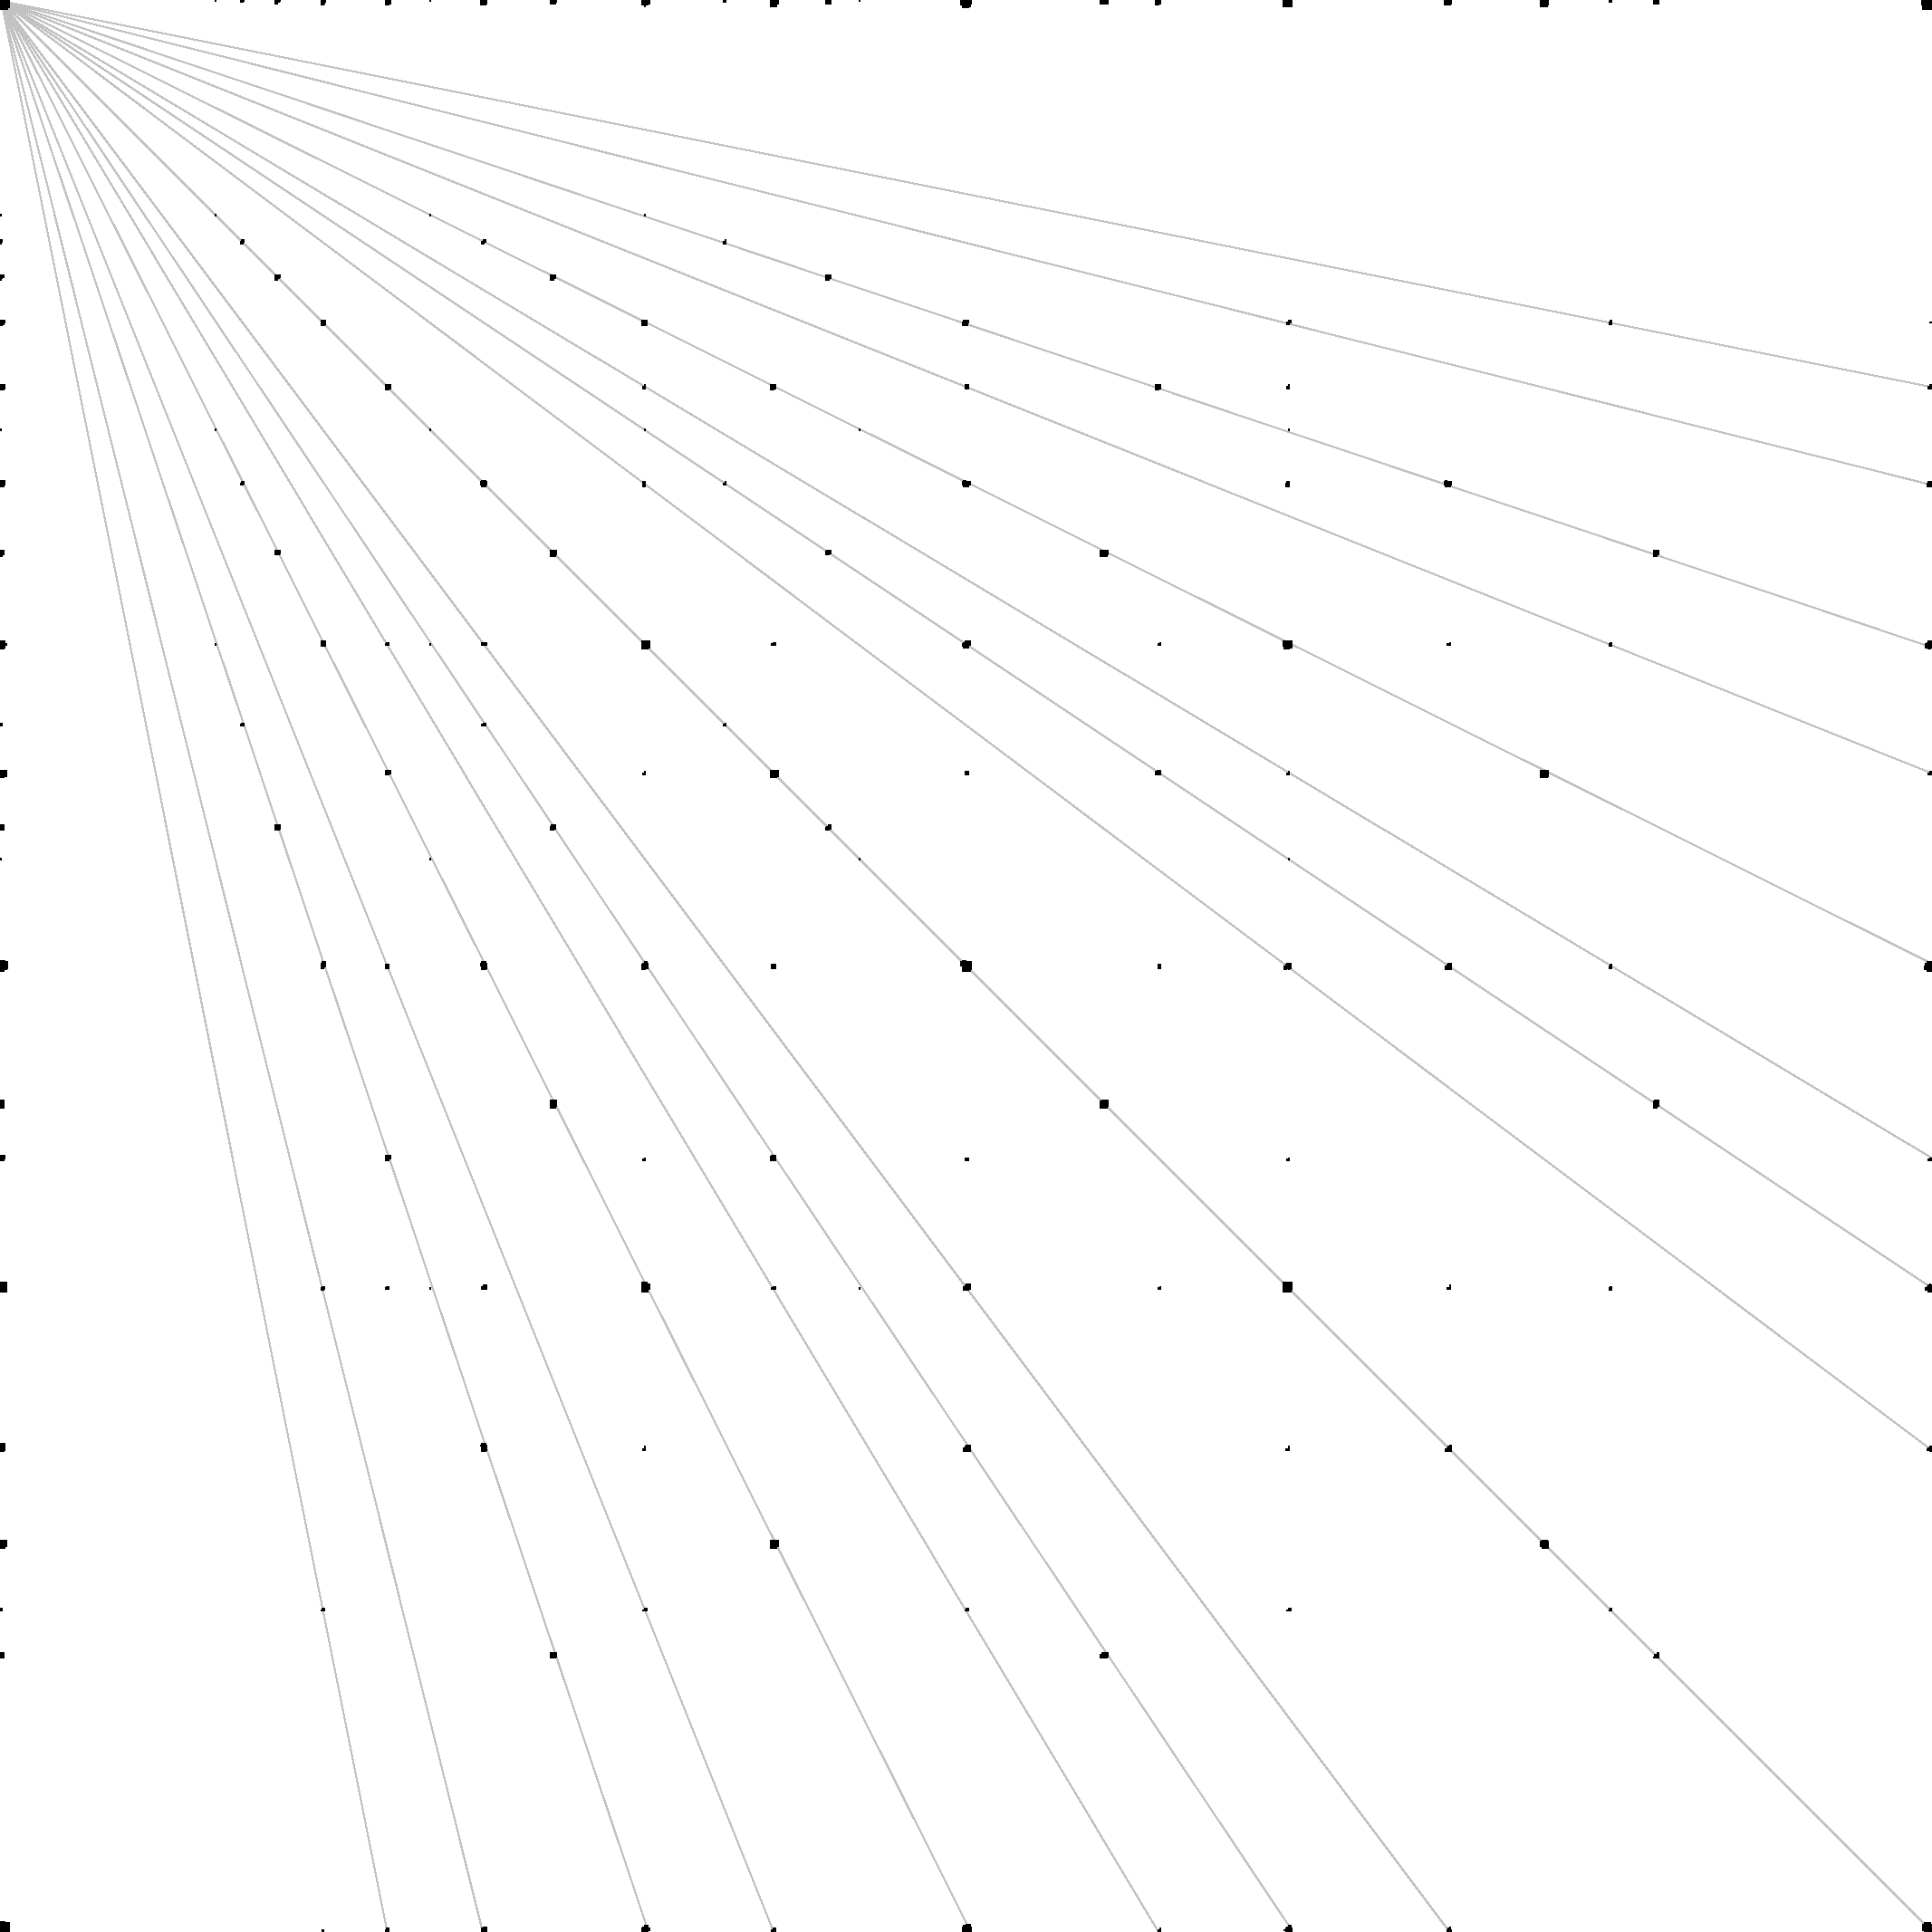
\includegraphics[width=0.90 \linewidth]{powerday3.pdf}
\end{center}\vspace{-0.1in}
\caption{All possible outcomes for the first two players in 3-player
  power days. These are the same games as the 3-player power hours,
  but at this scale makes it clear the groupings and their sparsity
  in the limit. Lines plotted from (0,0) to (60,*) and (*,60) show
  significant structure, but don't explain some of the interior points.
  (TODO: what are these games? what did the other player drink?)
}
\label{fig:powerday3}
\end{figure}


\section{Generalized BMML}

\begin{figure}
\begin{center}
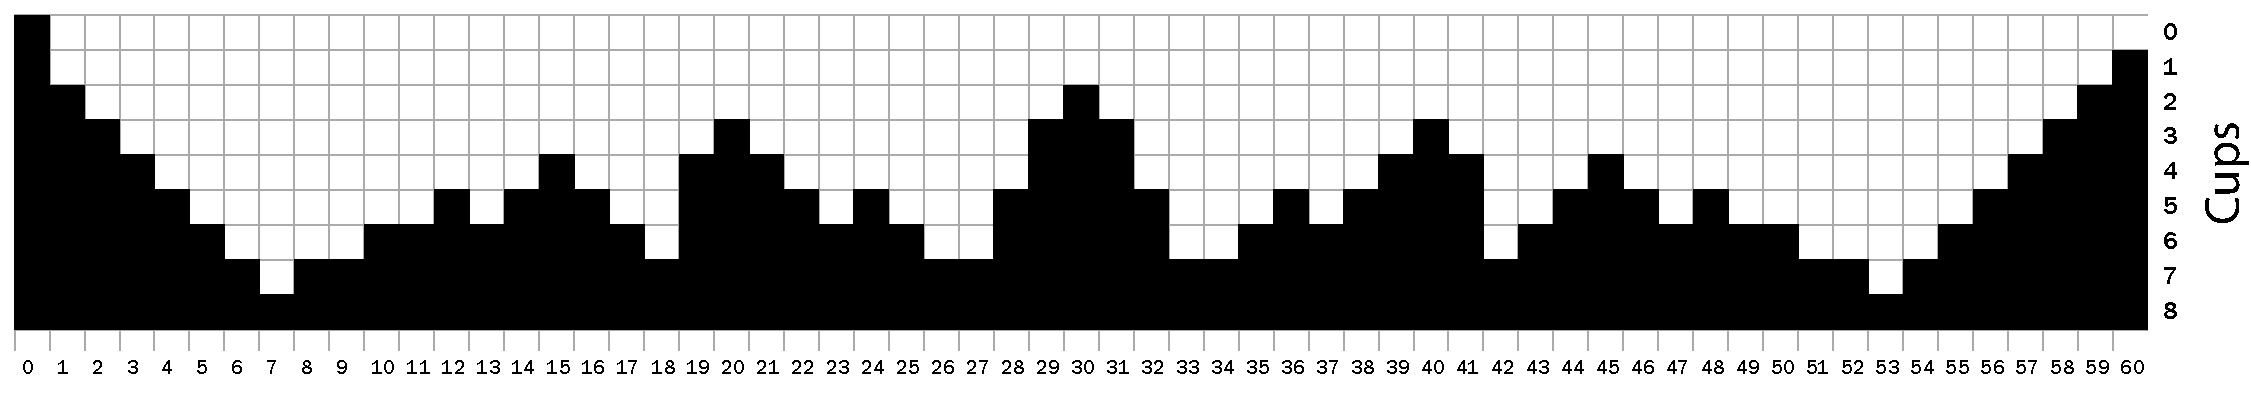
\includegraphics[width=0.90 \linewidth]{soloncups.pdf}
\end{center}\vspace{-0.1in}
\caption{Possible outcomes for BM$n$L with a single player. With no
  cup states, it is only possible to drink nothing. By convention, the
  0\th\ cup is the special ``filled'' state, so it is only possible to
  drink on every turn (60) or never (0). As we add more cup states,
  the number of achievable states strictly increases; with 8 cup states
  we can drink any amount. 7 and 53 drinks are the most difficult to
  achieve, and can only be done with 8 cup states.
}
\label{fig:soloncups}
\end{figure}


\begin{figure}
\begin{center}
\includegraphics[width=0.90 \linewidth]{composite2playermock.png}
\end{center}\vspace{-0.1in}
\caption{What's achievable for the first two players in a three-player
  generalized BM$n$L game, with $n$ ranging from 1 cup state (darkest)
  to 5 (lightest). TODO WRITEME
% 6 cupstates ran overnight and got here:
% #26186200000 queue 109 min 49 466729 states/sec 796272 config/sec
}
\label{fig:composite2player}
\end{figure}


\section{Known bounds}

Define BMnL, where $n$ is the number of non-filled states. BMML=BM2L.
Find $n$ such that a solo or dual power hour achieves any $k$.

\section{Conjectures} \label{sec:conjectures}

With two friends, you can drink any amount

Teetotaller: When $\langle k_1, \ldots, k_i, \ldots, k_n \rangle$ is possible,
so is $\langle k_1, \ldots, 0, \ldots, k_n \rangle$ (under what conditions)?

\section{Some stuffff}

Hi




\bibliography{paper}{}
\bibliographystyle{plain}
\end{document}
